\documentclass[a4paper,fontsize=14pt]{article}

\usepackage{cmap} %поиск в PDF
\usepackage[T2A]{fontenc}
\usepackage[utf8]{inputenc}
\usepackage[russian]{babel}
\usepackage[14pt]{extsizes}
\usepackage[left=35mm,right=10mm,
top=20mm,bottom=20mm,bindingoffset=0cm]{geometry}
\usepackage{listings}
\lstset{language=Python}
\lstset{frame=lines}
\lstset{caption={Insert code directly in your document}}
\lstset{label={lst:code_direct}}
\lstset{basicstyle=\footnotesize}

\usepackage[tocflat]{tocstyle}

\usepackage{graphicx}
\graphicspath{ {./images/} }


\begin{document}
	
	\begin{titlepage}
		\newpage
		
		\begin{center}
			Санкт-Петербургский политехнический университет Петра Великого \\
			Институт прикладной математики и механики \\
			\textbf{Высшая школа теоретической механики}
		\end{center}
		
		\vspace{10em}
		
		\begin{center}
			\Large{\textbf{Лабораторная работа №3}} \\
			Уравнение Лапласа. Вариант 6. \\
		\end{center}
		
		\vspace{20em}
		
		
		
		\newbox{\lbox}
		\savebox{\lbox}{\hbox{Е.Ю. Витохин}}
		\newlength{\maxl}
		\setlength{\maxl}{\wd\lbox}
		\hfill\parbox{12cm}{
			\hspace*{5cm}\hspace*{-5cm}Студент:\hfill\hbox to\maxl{А.А. Дурнев\hfill}\\
			\hspace*{5cm}\hspace*{-5cm}Преподаватель:\hfill\hbox to\maxl{Е.Ю.Витохин}\\
			\\
		}
		
		
		\vspace{\fill}
		
		\begin{center}
			Санкт-Петербург \\2020
		\end{center}
		
	\end{titlepage}
	
	\tableofcontents
	
	\newpage
	
	\section{Постановка задачи}
	
	Необходимо, используя метод конечных разностей, составить приближённое решение задачи Дирихле для уравнения Лапласа в квадрате $ABCD$ с вершинами $A(0, 0), \; B(0, 1), \: C(1, 1), \: D(1, 0)$. Шаг: $h = 0.2$, точность: $\epsilon = 0.01$. \\
	
	\begin{equation}
	\frac{\partial^2 u}{\partial x^2} + \frac{\partial^2 u}{\partial y^2} = 0
	\end{equation}

	где $x, \: y$ - пространственные координаты.\\
	
	Граничные условия:
	
	\begin{equation}
	U|_{AB} = 30sin(\pi y), \: U|_{BC} = 20x, \: U|_{CD} = 20y, \: U|_{AD} = 30x(1-x)
	\end{equation}
	
	
	Для численного решения уравнения будем использовать итерационный метод последовательных релаксаций.

	\section{Описание метода}
	
	Задаём сетки по осям $x$ и $y$:
	\begin{equation}
		y_j = jh,\; j=0,\dots,N	
	\end{equation}
	\begin{equation}
		x_i=ih, \; i=0,\dots,N
	\end{equation}
	
	$h$ - шаг сетки по осям $x$ и $y$, $N$ - количество узлов сетки по осям $x$ и $y$. \\
	
	Производные приближаем конечными разностями: \\
	\begin{equation}
		\frac{\partial^2 U}{\partial x^2} = \frac{U_{i-1,\:j} - 2U_{i,\:j} + U_{i+1,\;j}}{h^2}
	\end{equation}
	\begin{equation}
		\frac{\partial^2 U}{\partial y^2} = \frac{U_{i-1,\:j} - 2U_{i,\:j} + U_{i+1,\;j}}{h^2}
	\end{equation} \\
	
	Подставляя (5) и (6) в уравнение (1) получаем: \\
	
	$$U_{i-1,j}-4U_{i,j}+U_{i+1,j}+U_{i,j-1}+U_{i,j+1}$$
	
	Откуда:
	
	$$U_{i,j} = \frac{U_{i-1, j} + U_{i+1, j} + U_{i, j-1} + U_{i, j+1}}{4}$$
	
	Обозначим:
	
	$$\tilde{U}_{i,j} = \frac{U_{i-1, j} + U_{i+1, j} + U_{i, j-1} + U_{i, j+1}}{4}$$
	
	Вычисления будем производить по формуле:
	
	\begin{equation}
		U_{i,j}^{k+1} = U_{i,j}^{k} + \omega(\tilde{U}_{i,j}^k - U_{i,j}^k)
	\end{equation} \\
	
	Параметр $\omega$ в формуле (7) может изменяться в пределах $[0.5,1.9)$.\\ 
	
	Производим вычисления пока не выполнено условие:
	
	$$max|U_{i,j}^{k+1} - U_{i,j}^k| \leq \epsilon$$
	
	\section{Описание результатов}
	
	Определим наилучший параметр по зависимости $k(\omega)$, где $k$ - количество шагов:
	
	\begin{figure}[h]
		\center{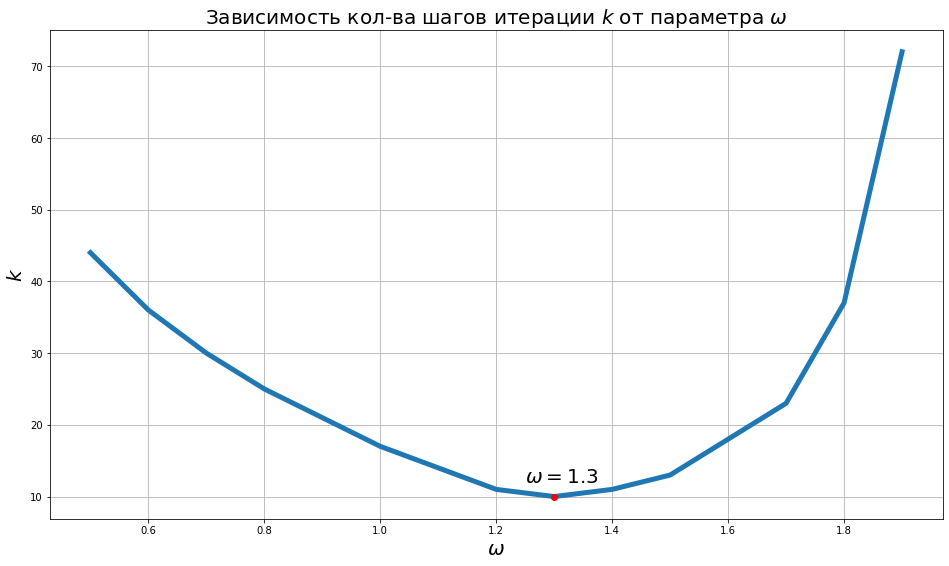
\includegraphics[scale=0.5]{pic1.png}}
		\label{pic1}
		\caption{}
	\end{figure}
	
	\newpage
	
	\begin{figure}[h]
		\center{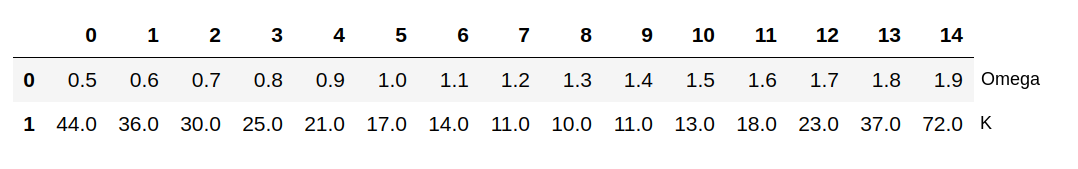
\includegraphics[scale=0.45]{pic3.png}}
		\label{pic1}
		\caption{Таблица с результатами $\omega$ и $k$}
	\end{figure}
	
	Решение при оптимальном параметре $\omega=1.3$:
	
	\begin{figure}[h]
		\center{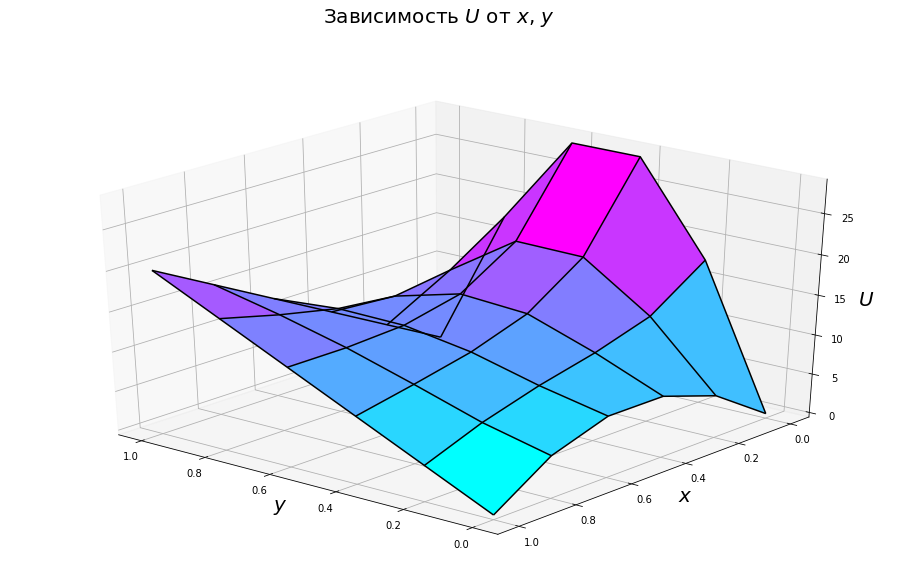
\includegraphics[scale=0.5]{pic2.png}}
		\label{pic2}
		\caption{}
	\end{figure}
	
	\newpage
	
	\begin{figure}[h]
	\center{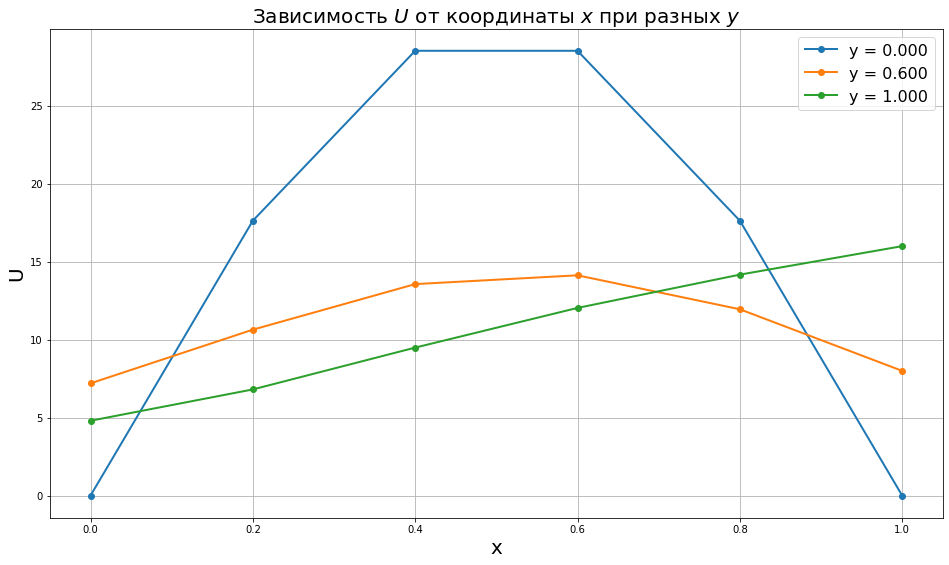
\includegraphics[scale=0.5]{pic5.png}}
	\label{pic2}
	\caption{}
\end{figure}

\newpage

\begin{figure}[h]
	\center{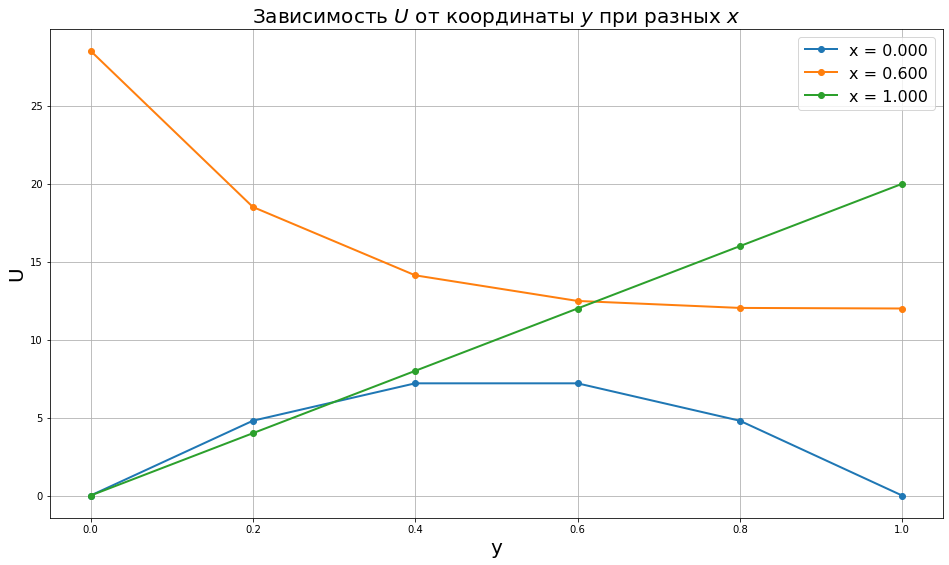
\includegraphics[scale=0.5]{pic6.png}}
	\label{pic2}
	\caption{}
\end{figure}

	\begin{figure}[h]
		\center{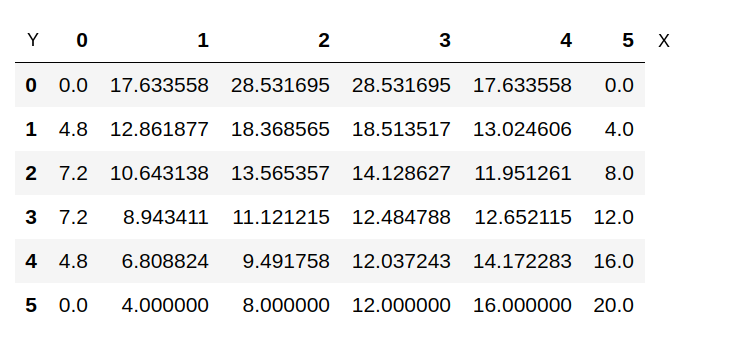
\includegraphics[scale=0.5]{pic4.png}}
		\label{pic2}
		\caption{Таблица с решением}
	\end{figure}

	
	\newpage
	
	\section{Приложение}
	
	Далее представлен код программы на Python: \\
	
	\lstinputlisting[language=Python]{code.py}
	
\end{document}